\subsection{The ITIL Framework}
\label{section:ITIL}
\ac{ITIL} is a framework and a source of good practice for service management, that is aligned with \acs{ISO}/\acs{IEC} 27000. This section gives a brief introduction to the \ac{ITIL} framework, focusing on the parts related to incident management and the content is, unless specified otherwise, derived from \cite{itilbok}. The definitions presented in this section are directly retrieved from \cite{itilbok}.

To describe service management, the \ac{ITIL} framework uses the following definitions:

\textbf{Service:} A service is a means of delivering value to customers by facilitating outcomes that customers want to achieve without the ownership of specific costs and risks.

\textbf{Service Management:} Service management is a set of specialized organizational capabilities for providing value to customers in the form of services.

The specialized organizational capabilities include the processes, activities, functions and roles that a service provider uses in delivering services. The \ac{ITIL} framework is generic and is meant to be useful for any type of organization. It describes a set of functions and processes that can be implemented in order to be able to perform service management. The terms function and process are defined in the following ways:

\textbf{Function:} A team or group of people and the tools they use to carry out one or more processes or activities.

\textbf{Process:} A process is a structured set of activities designed to accomplish a specific objective. A process takes one or more defined inputs and turns them into defined outputs. A process may include any of the roles, responsibilities, tools and management controls required to reliably deliver the outputs. A process may define policies, standards, guidelines, activities and work instructions if they are needed.

%Risk is defined as a possible event that could cause harm or loss, or affect the ability to achieve objectives. Risk can also be defined as the uncertainty of outcome.

This section describes processes and functions related to incident management.

\paragraph{Availability Management}
Availability management is essential for an organization and is primarily a proactive process. In addition to activities such as preparing and maintaining an availability plan and monitoring availability levels, this process includes assisting investigation and resolution of availability related incidents and problems. The latter is a reactive part of availability management. This process is related to other processes including IT service continuity, information security, event, incident and problem management.

\paragraph{IT Service Continuity Management}
This process is concerned with key systems in the event of a failure. The purpose of the process is to ensure that IT resources, systems and services can be restored within agreed timescales in the event of a major incident. The process is related to availability and information security management.

\paragraph{Information Security Management}
This process is concerned with enforcing the security policy. The system in place for this is the \ac{ISMS}. The security policy in an organization is something everyone should have access to and be aware of. Information security management is related to availability, incident, problem and IT service continuity management. 

\paragraph{The Service Desk}
The service desk is a function. One of the processes the service desk carries out is incident management. The service desk should be the single point of contact for IT users in an organization. This means that if users wish to log incidents or report events they should contact the service desk. The service desk is the owner of incidents throughout their lifecycle, regardless of who is working on the incident. They should be trained to obtain the skills needed in order to perform incident management as effectively and efficiently as possible.

\paragraph{Incident Management}
This is the process for dealing with incidents. An incident is defined as being an unplanned interruption or reduction in quality of an IT service. An incident can also be the failure of a configuration item that has not yet impacted service. Hence, incident management includes both incidents where service has been disrupted or where service has not yet been disrupted. Each organization should have its own definition of a major incident. Large organizations may have dedicated teams available 24/7 to handle major incidents. 

\begin{sidewaysfigure}
\centering
\scalebox{0.45}
{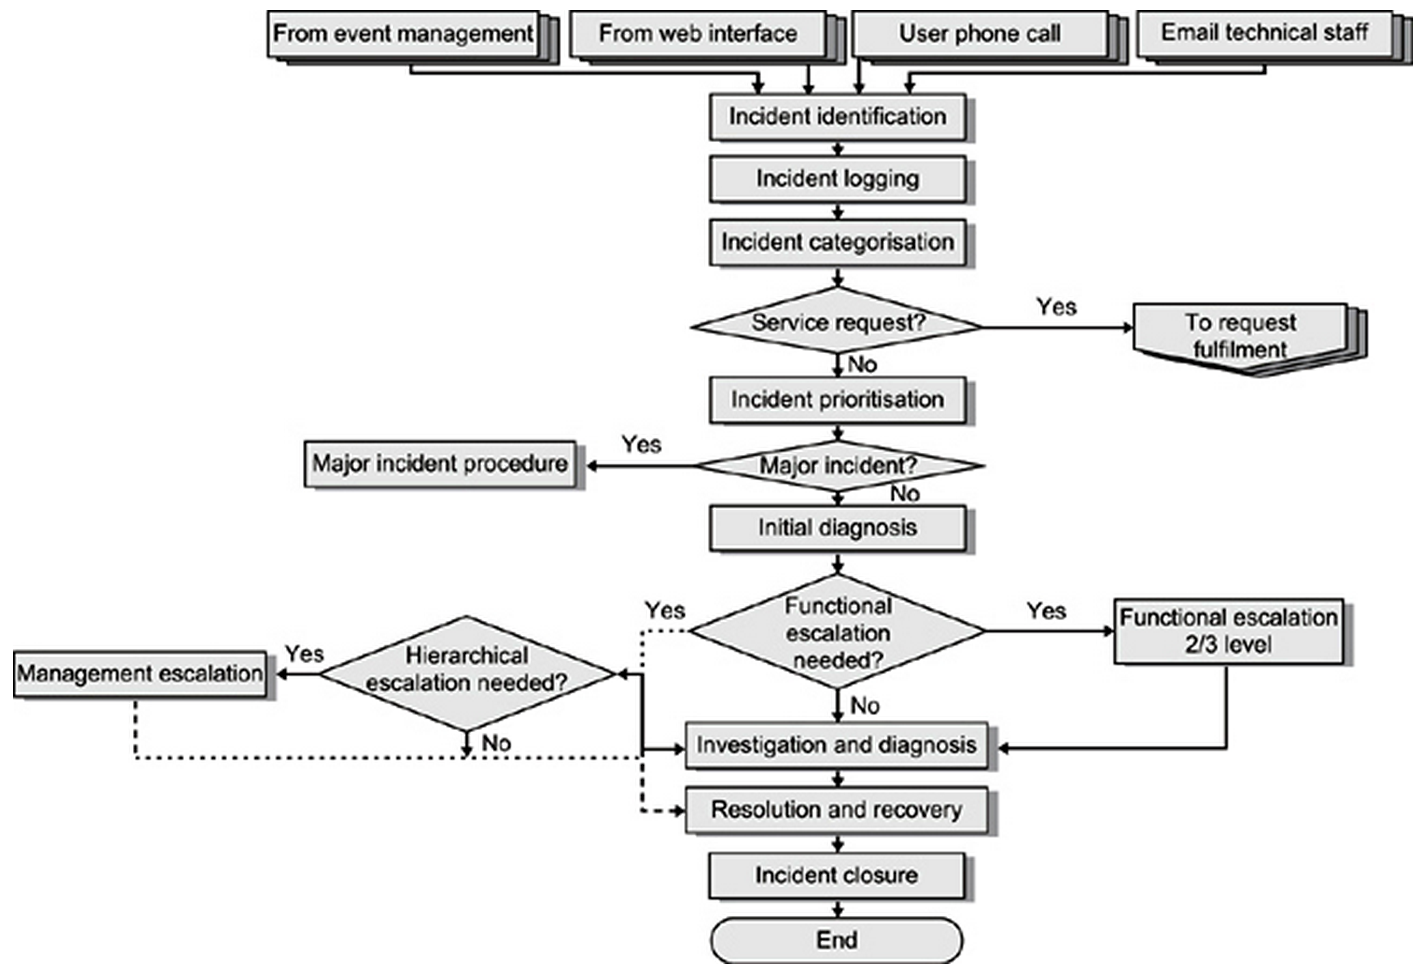
\includegraphics{ITILIncidentManagement.png}}
\caption[The ITIL Incident Management Process]{Incident Management Process \cite{itilbok}} 
\label{fig:ITILIncidentManagement}
\end{sidewaysfigure}

\pagebreak
In the incident management process resources are allocated to minimize and mitigate the impact of incidents and service unavailability in line with business priorities. The main objectives are to restore service as quickly as possible in addition to limit adverse impact on business operations. Incident handling may reveal areas that are in need of improvement. Organizations can adopt incident models, which are methods for handling groups of similar incidents.

The incident management process flow is illustrated in figure \ref{fig:ITILIncidentManagement}. The figure shows that incident reports can come from various sources. The incident reported needs to be identified, logged, categorized and prioritized. Accurate categorization is important as areas of the infrastructure where incidents occur can be highlighted. An example of an incident priority coding system can be seen in figure \ref{fig:ITILIncidentPrioritization}.

\begin{figure}[ht]
\begin{center}
\hspace{-0.2cm}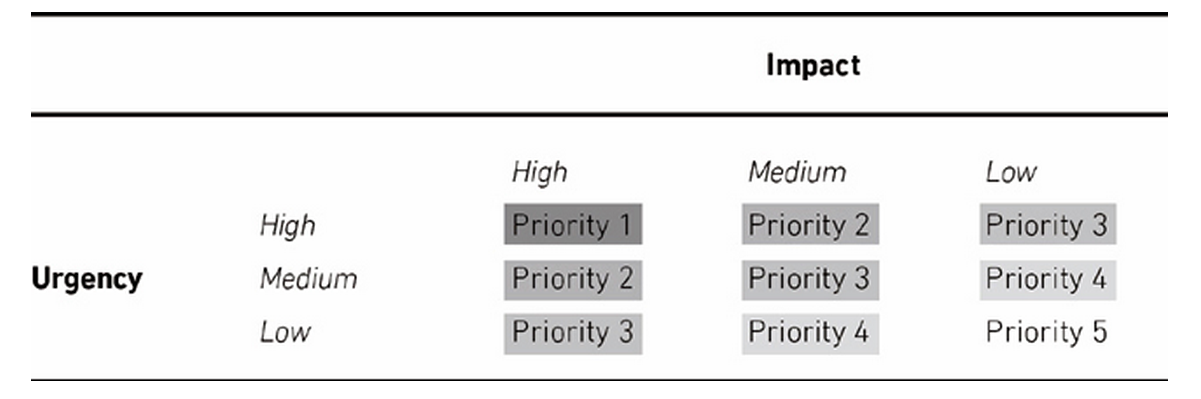
\includegraphics[scale=0.4]{ITILIncidentPrioritization.png}
\caption[ITIL Incident Priority Coding System]{Incident Priority Coding System \cite{itilbok}}
\label{fig:ITILIncidentPrioritization}
\end{center}
\end{figure}

If the incident turns out to be major, the major incident process is initiated. The incident handling may also need to be escalated. Functional escalation is when the service desk is not able to resolve the incident or when they have not been able to resolve it within the target resolution time. Hierarchical escalation is when the profile of a specific incident within the IT organization and also within business areas needs to be raised. Any incident needs to be investigated and diagnosed in order to subsequently be resolved and closed. The incident management process is closely related to the problem management process.

\begin{figure}[H]
\hspace{-1cm}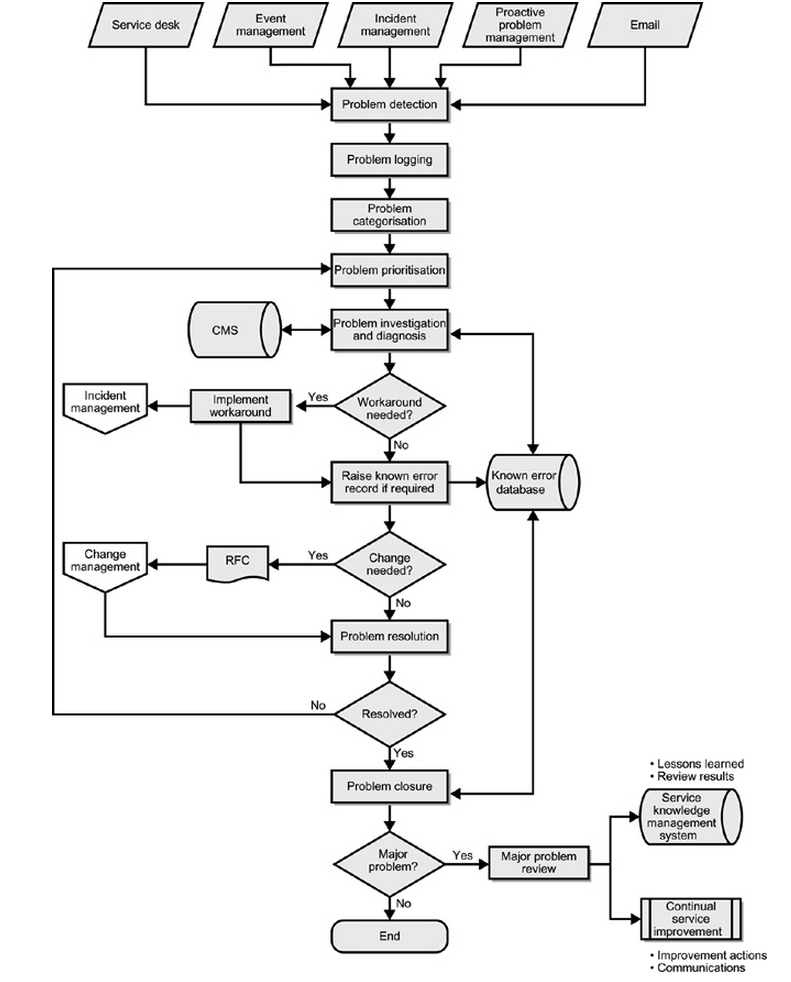
\includegraphics[scale=0.68]{ITILProblemManagement.png}
\caption[The ITIL Problem Management Process]{Problem Management Process \cite{itilbok}}
\label{fig:ITILProblemManagement}
\end{figure}

\paragraph{Problem Management}
The problem management process concerns analysis of the root cause as well as the resolving of problems. A problem is defined as being the cause of one or more incidents. The process is both proactive and reactive and seeks to prevent problems and incidents as well as reduce the impact of those that cannot be prevented. The problem management process is illustrated in figure \ref{fig:ITILProblemManagement}. 

The figure shows the various inputs to the process. It is important to log all details of the problem. Each problem needs to be categorized and prioritized. They should be prioritized in the same way as incidents, e.g. as in figure \ref{fig:ITILIncidentPrioritization}. During investigation and diagnosis the root cause of the problem should be discovered. The problem needs to be resolved as soon as a permanent fix is available and subsequently closed. If the problem is major, a major problem review must be conducted.

\paragraph{Event Management}
The event management process handles normal messages and detects, escalates and reacts to exceptions. An event can be informational, a warning or an exception. The event management process is similar to the incident management process and should ideally be automated. Some events are triggers for the incident management process.
%CI - Configuration Item